\section{Influence and diagnostic plots for \loglin\ models}\label{sec:loglin-infl}

Model diagnostic statistics
provide important ancillary information regarding the adequacy of
a \loglin\ model as a true summary of the relationships among the
variables
captured in the data.
As in logistic regression models (see \secref{sec:logist-infl}),
there are analogs of leverage, Cook's D, and the
leave-one-out \(\Delta \chi^2\) statistics for \loglin\ models,
described in \secref{sec:loglin-inflcat}.
Half-normal plots (\secref{sec:loglin-halfnorm})
are particularly useful for detecting outlier cells.

Most of the basic diagnostic quantities are calculated by \PROC{GENMOD}
and made available for plotting by use of the statement
\pname{make 'obstats' out=}%
\footnote{\sasver{7} uses the Output Delivery System with the
\stmt{ODS}{GENMOD} instead.}
and the options
\pname{obstats residuals} on the \stmt{MODEL}{GENMOD}.
A macro program, \pname{INFLGLIM} (\secref{loglin-inflglim}), 
is provided for calculating
additional diagnostics (hat values and Cook's D) that are not
supplied by \PROC{GENMOD} and for producing useful plots of these
measures.
For models which can be fit using \PROC{GENMOD}, the
\macro{INFLGLIM} makes model diagnosis easy.

These diagnostic quantities are not computed by \PROC{CATMOD};
however, with some effort,
they may also be obtained from the results of \PROC{CATMOD}, as described
in \secref{sec:loglin-inflcat}.

\subsection{Residuals and diagnostics for \loglin\ models}\label{sec:loglin-resids}

For a \loglin\ model, the simple, raw residual in cell $i$ is
$e_i \equiv n_i - \widehat{m}_i$.
But this is of little use because, with $n_i$ distributed as
$\Pois ( m_i)$, the variance of $n_i$ is $m_i$,
so cells with larger expected frequencies will have larger raw
residuals.
As a result, it is common to standardize by dividing by $\sqrt{ \widehat{m}_i}$,
giving the \glossterm{Pearson residual},
\begin{equation*}%\label{eq:reschi3}
r_i \equiv \frac{n_i - \widehat{m}_i}{\sqrt{ \widehat{m}_i}} \comma
\end{equation*}
which again are components of the overall Pearson \chisq, in the
sense that $\chisq = \sum r_i^2$.

For a good-fitting model, one might expect these so-called
``standardized'' residuals to have a normal distribution
with mean 0 and variance 1, that is, $\vec{e} \sim N ( \vec{0}, \sigma^2 \mat{I} )$.
But this expectation ignores the facts that parameters have been
estimated,
and the estimated residuals have degrees of freedom equal to
the residual df = (number of cells) - (number of parameters).%
\footnote{Following \citet{Christensen:97}, a better term
would be ``crude standardized residuals''.}
When the constraints on the residuals are taken into account,
it turns out (\citet[Section 12.4]{Agresti:90},
\citet[Section 10.7]{Christensen:97})
that the Pearson residuals for a correct \loglin\ model are
distributed asymptotically with standard errors
\begin{equation*}%\label{eq:seres}
\hat{\sigma} ( r_i ) = \sqrt{ 1 - h_{ii} }
\end{equation*}
where $h_{ii}$ is the leverage or hat value defined in \eqref{eq:hat-glim} below.%
\footnote{This is similar to the situation in ordinary linear models,
where the estimated residuals are distributed $N ( \vec{0}, \sigma^2 (\mat{I} - \mat{H})$, and so have standard errors equal to $\sqrt{ 1 - h_{ii} }$.}
Consequently, one may define \glossterm{adjusted residuals} \citep{Haberman:73,Haberman:74},
\begin{equation}\label{eq:streschi}
r_i^{\star} \equiv \frac{n_i - \widehat{m}_i}{\sqrt{ \widehat{m}_i ( 1 - h_{ii} )} } \comma
\end{equation}
which are standardized to have unit asymptotic variance.
Cells with large expected frequencies tend to have large hat values,
and hence, small standard errors.
The effect of ignoring the adjustment is therefore to underestimate
the magnitude of residuals in cells with large expected frequency.
We illustrate this effect in \exref{ex:berkeley9} below.

From the perspective of maximum likelihood estimation,
\glossterm{deviance residuals} may be defined as
\begin{equation}\label{eq:resdevg}
g_i  =
\mbox{sign} ( e_i ) \: \left[ 2
| n_i \log ( n_i / \widehat{m}_i ) | +  ( n_i - \widehat{m}_i ) \right] ^{1 / 2}
 \comma
\end{equation}
the signed
square root of the contribution of cell $i$ to the \LR\ \GSQ\
(or deviance), so that $\GSQ\ = \sum g_i^2$.
Analogous \emph{adjusted deviance residuals}, $g_i^{\star}$, are defined by dividing
$g_i$ by $\sqrt{ 1 - h_{ii}}$.

For any generalized linear model,  the
hat value, $h_{ii}$ may be calculated
as the $i$-th diagonal element of the matrix
\begin{equation}\label{eq:hat-glim}
\mat{H} = {\mat{W}}^\frac{1}{2} \mat{X}
{( \mat{X}\trans \mat{W} \mat{X})}^{-1} \mat{X}\trans  {\mat{W}}^\frac{1}{2}
 \comma
\end{equation}
where $\mat{W}$ is the diagonal matrix of weights used in computing
the Hessian.  For \loglin\ models, $\mat{W} = \diag (\vec{m})$.

Various measures of influence for logistic regression  (\secref{sec:logist-infldiag}) were defined to measure the effect
of deleting each observation on model fit statistics or estimated
parameters.  Similar diagnostics for \loglin\ models may be
defined for the contributions of each cell.

Cook's distance, $C_i$, is a squared measure of the
impact the $i$th cell has on the estimated parameters, and hence on
the fitted frequencies.
For a \loglin\ model, imagine that we drop
each cell in turn, fit the model to the remaining cells,
and estimate the expected frequency for the omitted cell.
It would be computationally intensive to calculate this by refitting
the model for each cell, but a simple one-step approximation
\citep[Section 10.7]{Christensen:97} may
be calculated as
\begin{equation}\label{eq:cookdlog}
C_i = \frac{r_i^2 h_{ii}} {k(1-h_{ii} )}
\end{equation}
where $k$ is the number of parameters estimated in the model.
This measure is equivalent to the statistic $\overline{C}_i$
defined for logistic regression \eqref{eq:cookd3} divided by $k$.

Similarly, one-step estimates of the change in deviance
and Pearson \chisq\ associated with deleting cell $i$ may be calculated
as
\begin{equation*}%\label{eq:difdevl}
  \Delta G_{(-i)}^2 = \frac{g_i^2}{1-h_{ii}} = (g_i^{\star})^2
  \comma
\end{equation*}
and
\begin{equation*}%\label{eq:difchil}
  \Delta \chi_{(-i)}^2 = \frac{r_i^2}{1-h_{ii}} = (r_i^{\star})^2
  \period
\end{equation*}

\subsection{Half-normal probability plots of residuals}\label{sec:loglin-halfnorm}
As we have just seen, the adjusted Pearson and deviance residuals have a standard normal
distribution (in large samples)
when the fitted model is correct.
This suggests that a plot of the ordered residuals, $r_{(i)}$, against the
corresponding approximate expected values of
an equal-sized sample (of $N$ \ctab\ cells, here) would have in a
normal distribution,
$z_{(i)} = \Phi^{-1} \{ (i-\frac{3}{8}) / ( N + \frac{1}{4}) \}$,
where $\Phi^{-1} (\bullet)$ is the inverse normal, or probit function.
Such plots, called \emph{normal quantile plots}
or \emph{normal QQ plots}, are commonly
used for GLMs with a quantitative response variable.
These plots are described in \SSSGref{3.5} and illustrated there in \S 5.4.2.

The graphical principle is that standardized residuals from a specified
distribution against quantiles from that distribution
should plot along a line through the origin with slope 1.
The \macro{NQPLOT} (see \SSSGref{\S A.1.10}) plots residuals against their
normal quantiles with a 95\% confidence envelope,
which makes it easier to determine when residuals stray far enough from
the line to be considered worrisome.

For generalized linear models, several enhancements to these ideas
have been suggested.
First, model departures and outliers are often easier to see for
discrete data when the \emph{absolute values} of residuals are plotted,
because large positive and negative values are sorted together.
This gives the \glossterm{half-normal plot}, in which the
absolute values of residuals,  arranged in increasing order, $|r|_{(i)}$,
are plotted
against
$|z|_{(i)} = \Phi^{-1} \{ (N+i-\frac{1}{8}) / (2N + \frac{1}{2}) \}$.
All outliers will then appear  in the upper right of such a plot,
as points separated from the trend of the remaining cells.

Second, the normal-theory reference line, $|r|_{(i)} = |z|_{(i)}$
and the normal-theory confidence envelope
may not be appropriate for generalized linear models
(or even ordinary linear models with small sample size).
\citet{Atkinson:81} proposed replacing these with a
\boldital{simulated envelope}, and reference line obtained by simulating residuals
from the assumed distribution.
These reference quantities are calculated in the following way for
a \loglin\ model.

For each cell, 19 additional observations are generated from a Poisson
distribution with mean $\widehat{m}_i$, the expected frequency in this cell
under the fitted model.
The same model fitted to the actual data is then fit to each of these
simulated \Dsets, giving a new set of residuals for each simulation.
For each set, sort the absolute residuals, and obtain the mean, minimum,
and maximum.
In the half-normal plot, the curve for the mean absolute simulated
residual serves as the data-based reference line instead of the normal-theory
line  $|r|_{(i)} = |z|_{(i)}$;
similarly, curves for the minimum and maximum of the 19 simulated
\Dsets\ may replace the normal=theory confidence limits.

The \macro{HALFNORM} (\macref{mac:halfnorm}) performs this simulation for
any generalized linear model fit with \PROC{GENMOD}
with the standard error distributions (normal, binomial, Poisson, gamma)
and produces a half-normal plot with the simulated mean and 95\%
reference curves.%
\footnote{\citet{FloresFlack:90} make the reasonable suggestion to replace the
mean, minimum and maximum, by resistant, but otherwise equivalent values,
namely, the median and median $\pm 1.5 \mbox{IQR}$, where IQR is the
interquartile range.
This suggestion is not yet implemented in the \macro{HALFNORM}.}
These plots are illustrated in the examples which follow.

\subsection{Model diagnostics with \PROC{GENMOD} and the \macro{INFLGLIM}}\label{loglin-inflglim}
The observation statistics calculated by \PROC{GENMOD}
include most of the residuals described for logistic regression models
in \secref{sec:logist-infl}, but they do not include the ``hat'' value
measure of leverage, or the influence measures, Cook's D ($C_i$), $\Delta G_{(-i)}^2$, and $\Delta \chi_{(-i)}^2$.

In terms of the variables in the \pname{OBSTATS} \Dset, the hat values,
$h_{ii}$, may be calculated as \pname{hat = Hesswgt * STD**2},
where \pname{STD} is the standard error of $\vec{x}_i\trans \vec{\beta}$.
Cook's D, as defined in \eqref{eq:cookdlog}, may be calculated as
\pname{cookd = hat * streschi**2 / (k*(1-hat))}, where \pname{streschi} is
the adjusted Pearson residual ($r_i^{\star}$), and \pname{k} is the
number of parameters in the model.  The value of \pname{k} may be
obtained from \PROC{GENMOD} as the sum of the \pname{DF} values in
the \pname{parmest} \Dset.

In addition, the \pname{OBSTATS} \Dset\ does not include the
factor (\pname{CLASS}) variables from the input \Dset,
so these variables must be merged with the \pname{OBSTATS} \Dset\ to
create plots in which the observations (cells of the \ctab)
are labeled meaningfully.

These calculations, and a variety of plots, are carried out by the
\macro{INFLGLIM} (see \macref{mac:inflglim}).  The following example
illustrates how to do these calculations directly, and the use of
the \macro{INFLGLIM}.
\begin{Example}[vietnam3]{Student opinion about the Vietnam war}
The revised model, with linear effects of year on each logit,
and with graduate students treated as \pname{yr=7}
 shown in \figref{fig:vietnam3} was fit using
\PROC{CATMOD}.  However, influence diagnostics are
easier to obtain using
\PROC{GENMOD}.
The same model can be fit using \PROC{GENMOD} by defining a dummy variable
for women and an interaction between \pname{yr} and a dummy variable
for men.
\begin{listing}
data vietnam;
   set vietnam;
   yr = year + 2*(year=5);
   mlin =  yr * (sex='M');
   female = (sex='F');
   cell = trim(sex)|| put(year,1.)|| trim(put(response,letter.));
   label yr="Year + 2(Grad)";

proc genmod data=vietnam;
   class year sex response;
   model count = year|sex response|mlin  response|female /
         dist=poisson obstats residuals;
   make 'obstats' out=obstats;
\end{listing}
Normally, one would need to merge the input \Dset\ with the \pname{obstats},
and calculate hat values, Cook's D or other quantities for plotting:
\begin{listing}
%let k=8;
data obstats;
   merge vietnam obstats;
   h = hesswgt * std**2;
   cookd = streschi**2 * h/((1-h) * &k);
\end{listing}
where \pname{k=8} is the number of estimated parameters.

Instead, the \macro{INFLGLIM} (\macref{mac:inflglim}) automates these steps, and
gives various influence plots of residuals from a given
model.  The macro plots all combinations of the variables given
by the \mparm{GY}{INFLGLIM} against the variables given by the \mparm{GX}{INFLGLIM},
using a bubble symbol whose size is proportional to the
\mparm{BUBBLE}{INFLGLIM}, usually Cook's D.

Here, we plot the one-step estimates of change in deviance
($\Delta G_{(-i)}^2$, or \pname{DIFDEV})
due to deleting each cell against hat values,
using bubble symbols with area proportional to Cook's D.
The \mparm{infl}{INFLGLIM} determines the criterion for labeling
potentially influential points.
\begin{listing}
%inflglim(data=vietnam, resp=count,
    class=year sex response,
    model= year|sex  response|mlin  response|female,
    dist=poisson, id=cell,
    infl=%str(difdev>4 or &bubble>1 or hat>1.5*&hcrit),
    gy=difdev, gx=hat, bubble=cookd);
\end{listing}

This plot (\figref{fig:vietgen3}) shows that there are still two
large residuals: 4th year men choose response B substantially less often
than predicted (accounting for over one-third of the model deviance), and first year women choose response C less than
predicted.
%% one figure
\begin{figure}[htb]
  \centering
  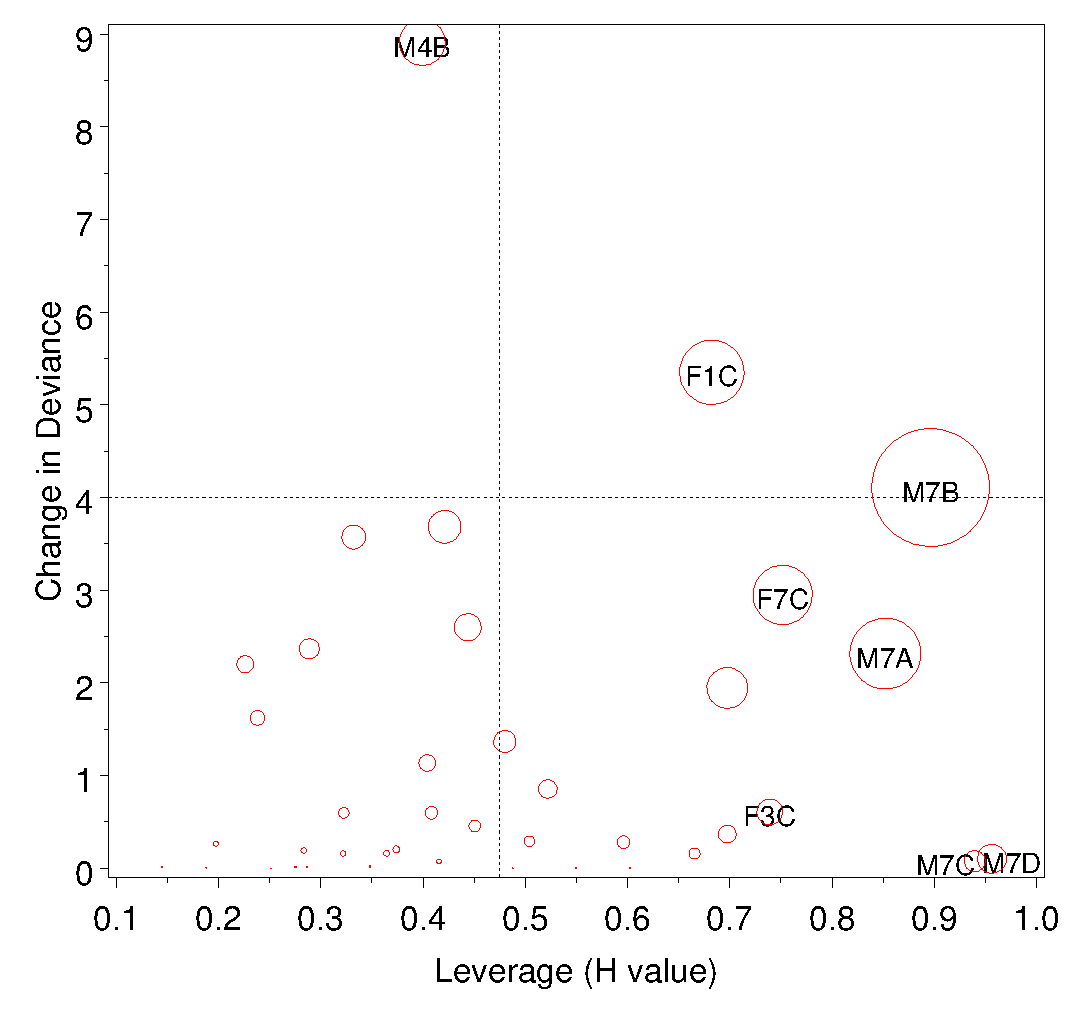
\includegraphics[scale=.6]{vietgen3}
  \caption{Influence plot for model $R = S + Y_{lin}(M)$, Graduate students=7}%
  \label{fig:vietgen3}
\end{figure}
We complete the analysis and this example with a half-normal plot of
these residuals, shown in \figref{fig:vietgen4}.  Although there is
evidence of non-normality in the distribution of residuals,  even the largest
values are within the simulated envelope.
\begin{listing}
%halfnorm(data=vietnam, resp=count,
   class=sex year response,
   model=year|sex  response|mlin  response|female,
   dist=poisson, id=cell);
\end{listing}

\begin{figure}[htb]
  \centering
  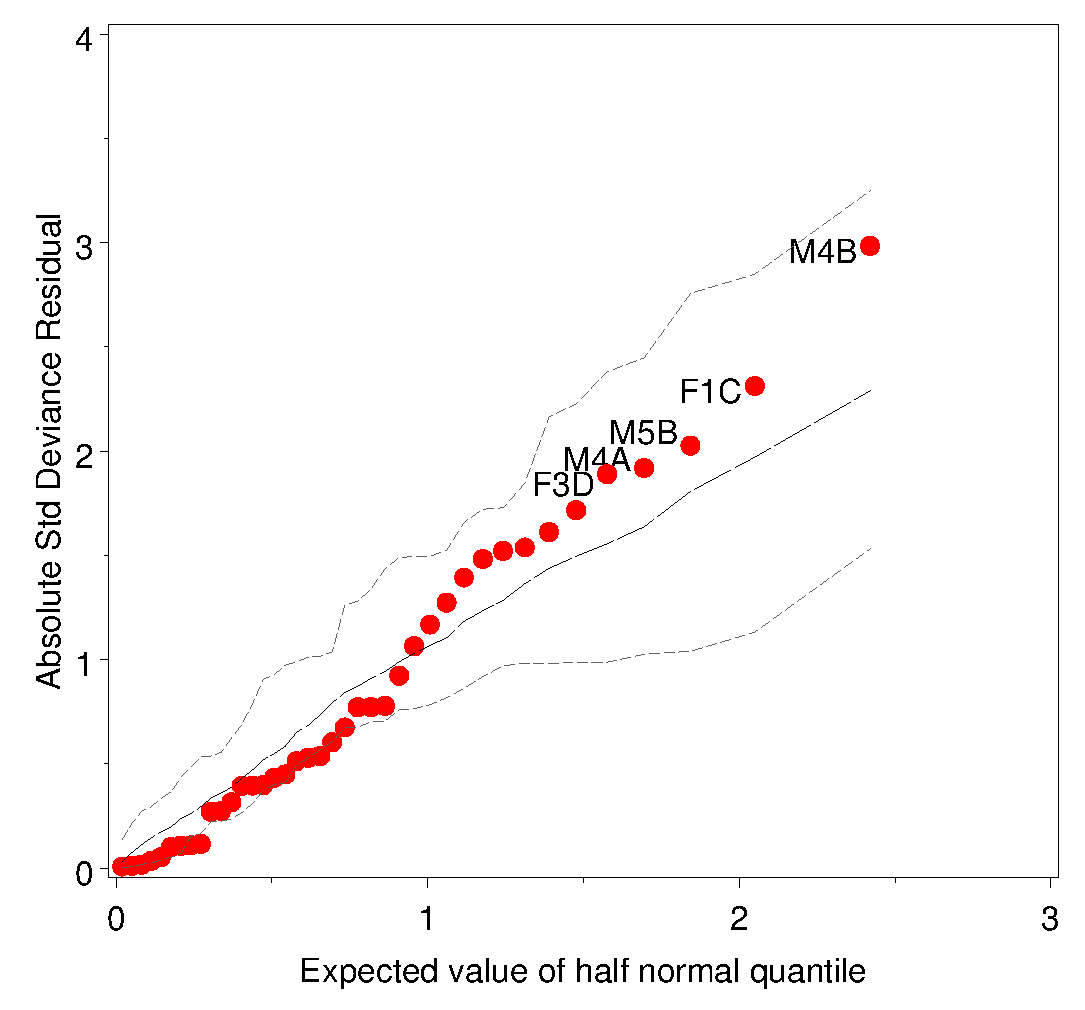
\includegraphics[scale=.6]{vietgen4}
  \caption{Half-normal plot for model $R = S + Y_{lin}(M)$, Graduate students=7}%
  \label{fig:vietgen4}
\end{figure}
\end{Example}


\begin{Example}[berkeley9]{Berkeley admissions}
These diagnostic plots may also be illustrated
with the Berkeley admissions
data using the \loglin\ model $[AD] [GD]$,
or the equivalent logit model, $\logit(\mbox{Admit}) = \alpha + \beta_i^{D}$.
Recall that we found this model fit well, except in department A.
To give useful labels for influential cells, we first combine the
factor variables into a character identifier, \pname{cell}.
\begin{listing}
data berkeley;
   set berkeley;
   cell = trim(put(dept,dept.)) ||
          gender ||
          trim(put(admit,yn.));
\end{listing}
We ask for an influence plot of adjusted Pearson residuals against hat values
(showing Cook's D by bubble size, by default):
\begin{listing}
%inflglim(data=berkeley, class=dept gender admit,
        resp=freq, model=admit|dept gender|dept, dist=poisson, id=cell,
        gx=hat, gy=streschi);
\end{listing}
The plot (\figref{fig:genberk11}) clearly indicates that the only cells
which do not fit ($|r_i| > 2$) are for department A.
Notice also, that the cells for males applying to this department
(with high expected frequencies)
have large leverage, and therefore large influence (Cook's D)
on this model.
%% one figure
\begin{figure}[htb]
  \centering
  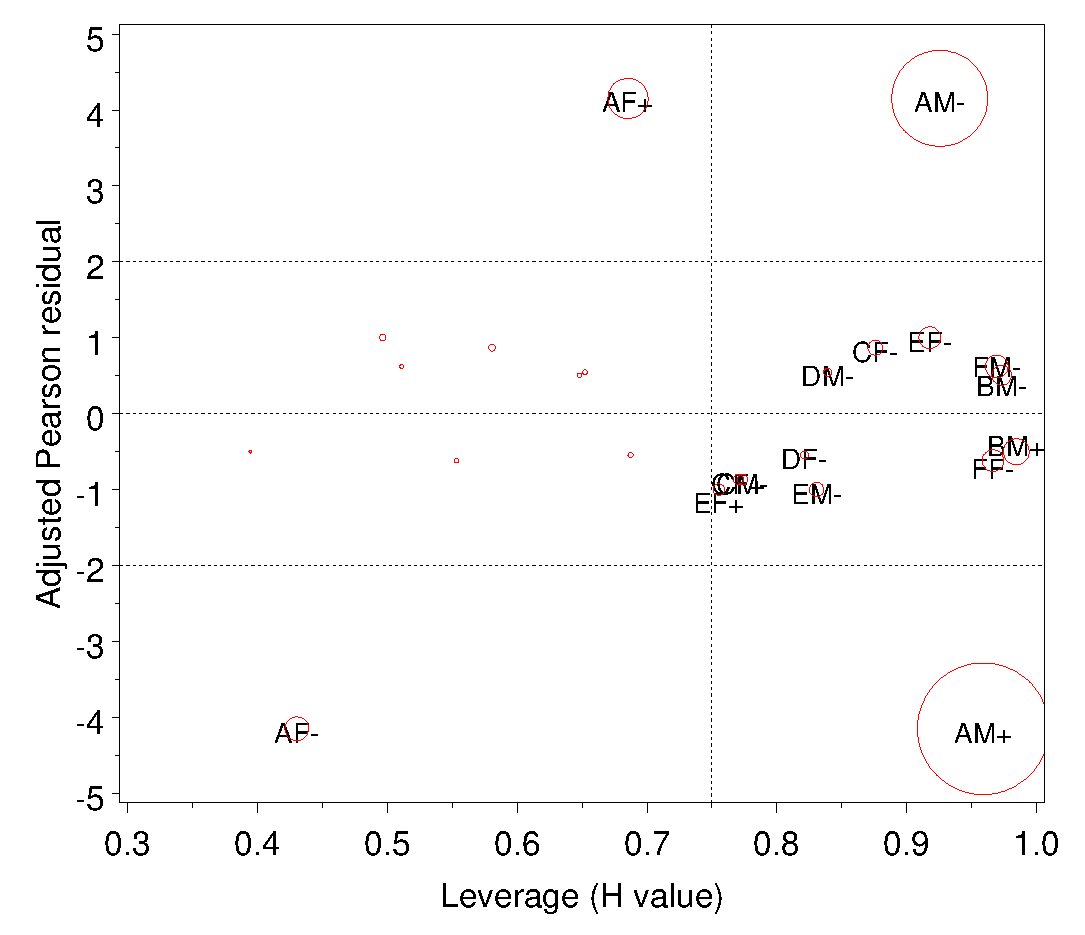
\includegraphics[scale=.6]{genberk11}
  \caption[Influence plot for Berkeley admissions data, Model AD GD]{Influence plot for Berkeley admissions data, Model $[AD] [GD]$.
  Bubble areas are proportional to Cook's D.}%
  \label{fig:genberk11}
\end{figure}

We can also illustrate why adjusted residuals are preferable to
the (crudely standardized) residuals by plotting the estimated
residual standard error, $\sqrt{1-h_{ii}}$ against fitted cell
frequency for this model.
This plot (\figref{fig:genberk12}) is produced as follows:
\begin{listing}
%inflglim(data=berkeley, class=dept gender admit,
        resp=freq, model=dept|gender dept|admit, dist=poisson, id=cell,
        gx=pred, gy=seres);
\end{listing}

%% one figure
\begin{figure}[htb]
  \centering
  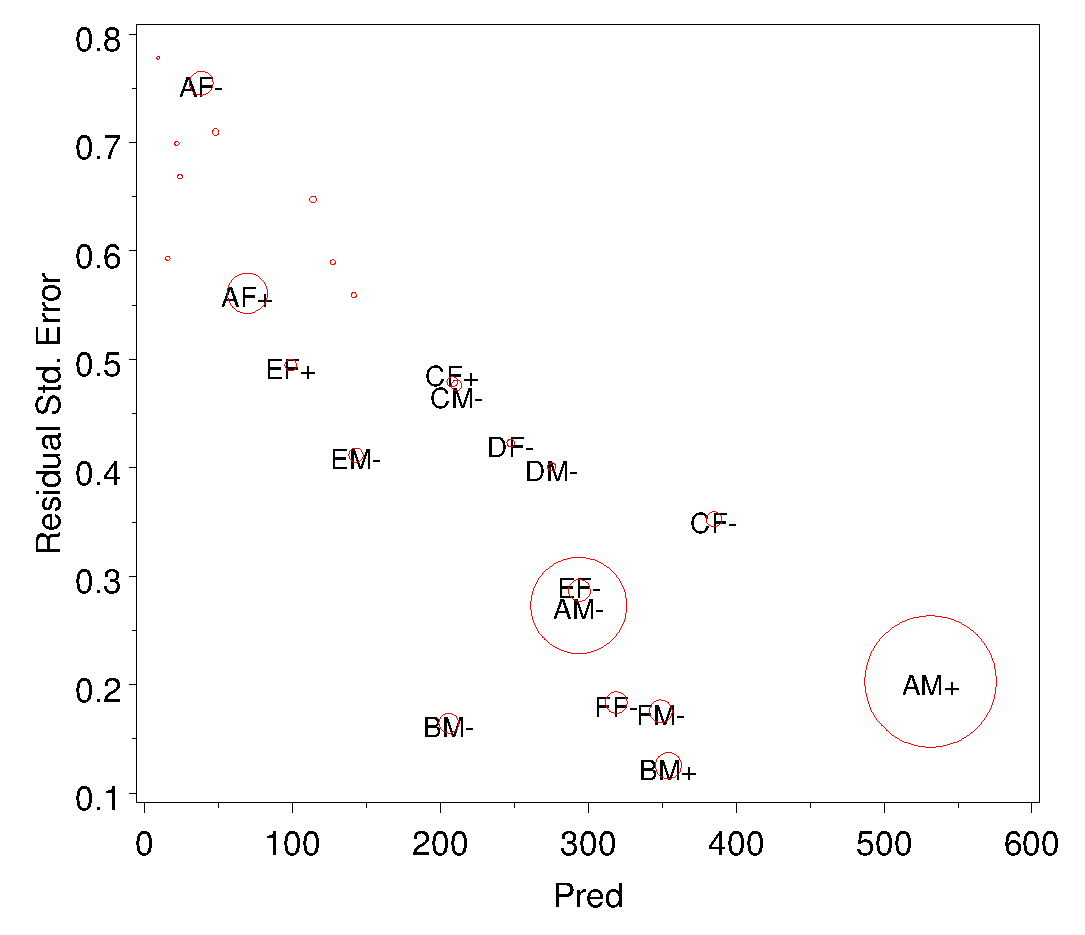
\includegraphics[scale=.6]{genberk12}
  \caption[Residual standard errors vs.\ fitted frequencies]{Residual standard errors vs.\ fitted frequencies for Berkeley admissions data, Model $[AD] [GD]$}%
  \label{fig:genberk12}
\end{figure}
We see that the standard errors decrease nearly linearly
with estimated expected frequency,
and the most influential cells (\pname{AM+} and \pname{AM-} for
males in Dept A)  have small standard errors,
and so their unadjusted residuals are most severely underestimated.
That is, cells with large expected frequency are
often highly influential, but their (unadjusted) residuals are
underestimated. 

Finally, we show a half-normal plot for this model in \figref{fig:genberk13},
produced with the \macro{HALFNORM},
\begin{listing}
%halfnorm(data=berkeley, class=dept gender admit,
   resp=freq, model=dept|gender dept|admit, dist=poisson, id=cell);
\end{listing}
By default, the cells with the largest 5 absolute residuals are labeled.
This plot clearly shows that the model fits well, except in department A.
%% one figure
\begin{figure}[htb]
  \centering
  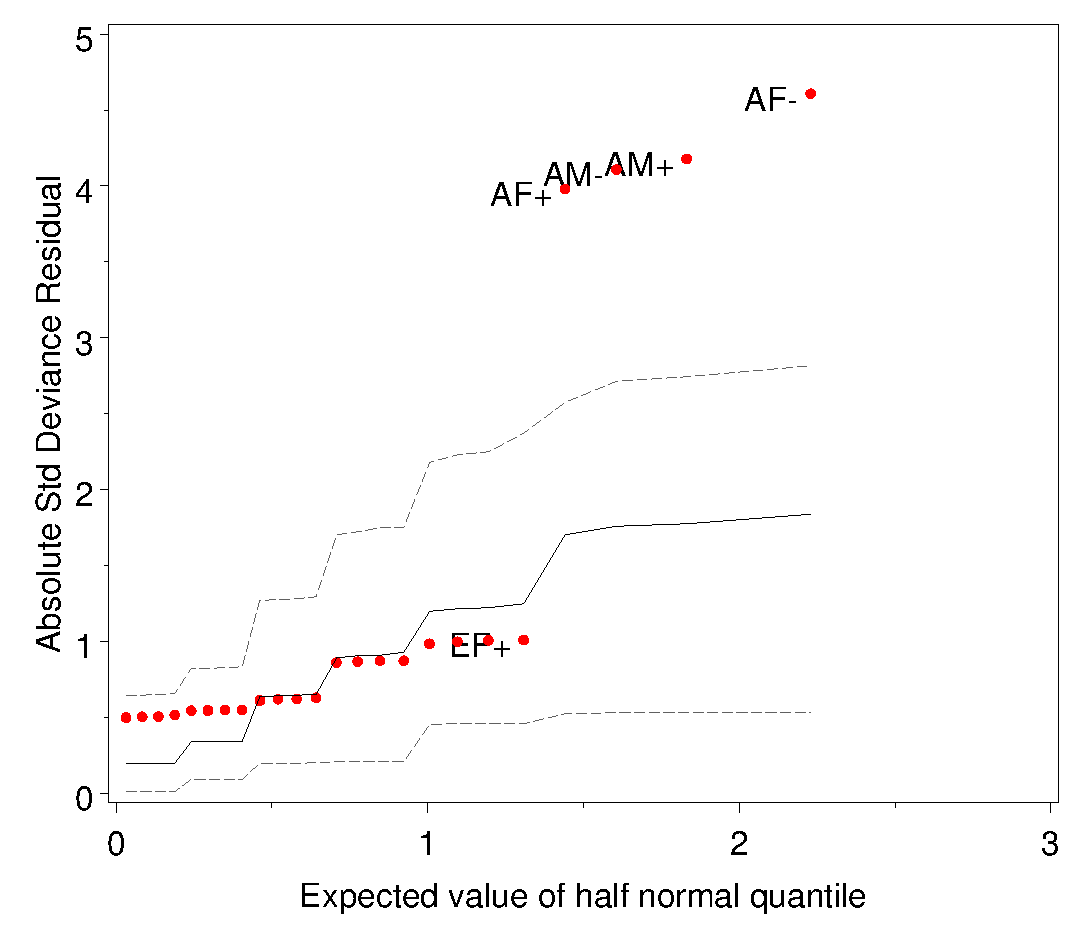
\includegraphics[scale=.6]{genberk13}
  \caption{Half-normal residual plot for Berkeley admissions data, Model $[AD] [GD]$}%
  \label{fig:genberk13}
\end{figure}
\end{Example}


\subsection{Model diagnostics with \PROC{CATMOD}}\label{sec:loglin-inflcat}

For situations where an equivalent model cannot be fit with \PROC{GENMOD},
the hat values and Cook's D can still be obtained from the \ODS\
from \PROC{CATMOD}.
The technique
described here is based on the idea \citep{Christensen:97}
that a \loglin\ model is essentially a regression model for log
frequency, which can be fit by weighted least squares regression.
The steps are:
\begin{enumerate}

\item Fit the \loglin\ model, obtaining the cell frequencies
	\(n_i\) and estimated expected frequencies \(\widehat{m}_i\) in a
	\Dset\ (see the statement {\tt RESPONSE / OUT=PREDICT}
	above).

\item Use \PROC{REG} to calculate a weighted regression and obtain
       the regression diagnostics (e.g., \pname{h} and \pname{cookd})
		 with an \stmt{OUTPUT}{REG}.  Fit the regression with:

	\begin{description}
	\item[independent variables:]  Dummy variables for all
			marginals and association terms in the \loglin\
			model. (\PROC{REG} does not provide a CLASS statement.)
	\item[dependent variable:]  The ``working'' response, \(y_i  =
			\log ( \widehat{m}_i )  +  ( n_i - \widehat{m}_i ) /  \widehat{m}_i\)
	\item[weights:]  \(\widehat{m}_i\)
	\end{description}

\item Leverages will be correctly reported in the output.  The
	adjusted residuals, however, will have been divided by
	\(\sqrt{MSE}\), and the Cook's D values will have been divided
	by \(MSE\).  For a model with \(k\) parameters and \(N\) cells
	the average leverage will be \(k/N\), so a value \(h_{ii} > 2 k
	/  N\) would be considered ``large''.

\end{enumerate}

\begin{Example}[berkeley10]{Berkeley admissions}
We continue with the results from model \([AD]  [GD]\),
to illustrate the computations with the results from \PROC{CATMOD}.
The expected frequencies were obtained
using the option \pname{PRED=FREQ} on the \stmt{MODEL}{CATMOD}, as 
\begin{listing}
proc catmod order=data data=berkeley;
   weight freq;
   model dept*gender*admit=_response_ /
         ml  noiter noresponse nodesign noprofile pred=freq ;
   response / out=predict;
   loglin admit|dept dept|gender / title='Model (AD,DG)';
\end{listing}
 In the \pname{PREDICT} \Dset, \(\widehat{m}_i\) is named
\verb|_PRED_|, \(n_i\) is \verb|_OBS_|, and \(e_i = n_i - \widehat{m}_i\)
is \verb|_RESID_|.
The working response may be calculated in a \Dstp\ as follows:
\begin{listing}
data rdat;
   set predict;
   drop _sample_ _type_ _number_;
   where (_type_='FREQ');
   cell = trim(put(dept,dept.)) ||
          gender ||
          trim(put(admit,yn.));
    *-- Working response;
   y = log(_pred_) + _resid_/_pred_;
\end{listing}
Fitting
the regression model for the working response using \PROC{REG} is
conceptually simple, though tedious because \PROC{REG} 
(like \PROC{LOGISTIC}) 
cannot generate the dummy variables itself.  This may be
done in a data step, or with \PROC{GLMMOD}, or using the
\macro{DUMMY} (\macref{mac:dummy}) and the \macro{INTERACT} (\macref{mac:interact}).
We illustrate using the macro programs; by default they append
the new variables to the input \Dset.
\begin{listing}
%dummy(data=rdat, var=admit gender dept, prefix=a g d);
%interact(v1=a0, v2=d1 d2 d3 d4 d5, prefix=ad);
%interact(v1=gf, v2=d1 d2 d3 d4 d5, prefix=gd);

proc reg data=rdat outest=est;
   id cell;
   weight _pred_;
   model y = a0 gf d1-d5 ad11-ad15 gd11-gd15;
   output out=regdiag
          h=hat cookd=cookd student=studres;
\end{listing}
In the final step, the $\sqrt{MSE}$ is obtained from the \pname{OUTEST}
\Dset, and the adjusted residuals and Cook's D may be calculated.
\begin{listing}
data regdiag;
   set regdiag;
   retain _rmse_;
   if _n_=1 then set est(keep=_rmse_ );
   adjres = studres * _rmse_;
   cookd = cookd * _rmse_**2;
\end{listing}
These quantities, shown in \outref{out:catberk4.1},
may then be plotted in the forms shown earlier using the
\macro{INFLGLIM}.

\begin{Output}[htb]
\caption{Diagnostics for the model $[AD][GD]$ calculated from \PROC{CATMOD} output}\label{out:catberk4.1}
\small
\verbatiminput{ch7/out/catberk4.1}
\end{Output}
\end{Example}



